\documentclass[nologo,a4paper,12pt]{article}

\usepackage[T1]{fontenc}
\usepackage[utf8]{inputenc}
\usepackage{lmodern}
\usepackage{microtype}
\usepackage[left=2.5cm,right=2.5cm,top=2.5cm,bottom=2.5cm,headheight=25pt]{geometry}
\usepackage{xcolor}
\usepackage{fancyhdr}
\usepackage{titlesec}
\usepackage{mdframed}
\usepackage{amsmath}
\usepackage{amssymb}
\usepackage{booktabs}
\usepackage{tabularx}
\usepackage{longtable}
\usepackage{array}
\usepackage{float}
\usepackage{parskip}
\usepackage{enumitem}
\usepackage{graphicx}
\usepackage{subcaption}
\usepackage{tikz}
\usetikzlibrary{arrows.meta}
\usepackage{hyperref}
\usepackage[capitalize]{cleveref}

\graphicspath{{figures/}{./}}

% left-aligned fixed-width column: avoids overfull lines in narrow table cells
\newcolumntype{P}[1]{>{\raggedright\arraybackslash}p{#1}}

\definecolor{mls@blue}{RGB}{0, 83, 134}
\definecolor{mls@gray}{RGB}{100, 100, 100}
\definecolor{mls@lightgray}{RGB}{245, 245, 245}
\definecolor{mls@green}{RGB}{40, 130, 60}
\definecolor{mls@lightgreen}{RGB}{220, 245, 225}
\definecolor{mls@red}{RGB}{160, 30, 30}
\definecolor{mls@lightyellow}{RGB}{255, 252, 220}
\definecolor{mls@yellow}{RGB}{180, 140, 0}
\definecolor{mls@lightblue}{RGB}{225, 238, 248}

\hypersetup{colorlinks=true,linkcolor=mls@blue,urlcolor=mls@blue}

% --------------------------------------------------------------------- header
\pagestyle{fancy}
\fancyhf{}
\fancyhead[L]{\small\color{mls@gray}Introduction to Machine Learning Safety}
\fancyhead[R]{\small\color{mls@gray}Safety Case Report}
\fancyfoot[C]{\small\color{mls@gray}\thepage}
\renewcommand{\headrulewidth}{0.6pt}
\renewcommand{\headrule}{{\color{mls@blue}\rule{\headwidth}{0.6pt}}}

% ------------------------------------------------------------------ sections
\titleformat{\section}{\large\bfseries\color{mls@blue}}{\thesection.\ }{0.4em}{}[{\color{mls@blue}\titlerule[0.6pt]}]
\titlespacing{\section}{0pt}{1.2em}{0.4em}
\titleformat{\subsection}{\normalsize\bfseries}{}{0em}{}
\titlespacing{\subsection}{0pt}{0.9em}{0.35em}

\setlength{\parskip}{0.35\baselineskip}
\setlength{\floatsep}{8pt plus 2pt minus 2pt}
\setlength{\textfloatsep}{10pt plus 2pt minus 2pt}
\setlength{\intextsep}{8pt plus 2pt minus 2pt}
\renewcommand{\topfraction}{0.9}
\renewcommand{\bottomfraction}{0.7}
\renewcommand{\textfraction}{0.08}
\renewcommand{\floatpagefraction}{0.8}

% ------------------------------------------------------------------ box styles
\mdfdefinestyle{claimstyle}{%
  backgroundcolor  = mls@lightgray,
  linecolor        = mls@blue,
  linewidth        = 2pt,
  topline          = false,
  rightline        = false,
  bottomline       = false,
  innerleftmargin  = 12pt,
  innerrightmargin = 10pt,
  innertopmargin   = 8pt,
  innerbottommargin= 8pt,
  skipabove        = 0.6em,
  skipbelow        = 0.6em,
}
\mdfdefinestyle{subclaim}{%
  backgroundcolor  = white,
  linecolor        = mls@blue,
  linewidth        = 0.8pt,
  roundcorner      = 3pt,
  innerleftmargin  = 10pt,
  innerrightmargin = 10pt,
  innertopmargin   = 6pt,
  innerbottommargin= 6pt,
  skipabove        = 0.9em,
  skipbelow        = 0.6em,
}
\mdfdefinestyle{evidencestyle}{%
  backgroundcolor  = mls@lightgreen!30,
  linecolor        = mls@green,
  linewidth        = 0.8pt,
  roundcorner      = 3pt,
  innerleftmargin  = 10pt,
  innerrightmargin = 10pt,
  innertopmargin   = 6pt,
  innerbottommargin= 6pt,
  skipabove        = 0.8em,
  skipbelow        = 0.6em,
}
\mdfdefinestyle{cautionstyle}{%
  backgroundcolor  = mls@lightyellow,
  linecolor        = mls@yellow,
  linewidth        = 2pt,
  topline          = false,
  rightline        = false,
  bottomline       = false,
  innerleftmargin  = 12pt,
  innerrightmargin = 10pt,
  innertopmargin   = 7pt,
  innerbottommargin= 7pt,
  skipabove        = 0.6em,
  skipbelow        = 0.6em,
}

\newcommand{\verdictmet}{\textbf{\color{mls@green}$\checkmark$~Met}}
\newcommand{\verdictnotmet}{\textbf{\color{mls@red}$\times$~Not met}}
\newcommand{\verdictpartial}{\textbf{\color{mls@yellow}$\approx$~Partial}}
\newcommand{\verdictunver}{\textbf{\color{mls@red}$\times$~Not verified}}
\newcommand{\verdictline}[1]{\textbf{Overall verdict:}\quad #1}

\newcommand{\yes}{{\color{mls@green}$\checkmark$}}
\newcommand{\no}{{\color{mls@red}$\times$}}
\newcommand{\maybe}{{\color{mls@yellow}$\approx$}}


\begin{document}


\begin{titlepage}
\thispagestyle{empty}
\centering
\vspace*{2.5cm}

{\color{mls@blue}\rule{\linewidth}{2pt}}\\[1.2em]
{\color{mls@blue}\Huge\bfseries Final Report}\\[0.8em]
{\LARGE Introduction to Machine Learning Safety}\\[0.6em]
{\large\color{mls@gray}CARLA Autonomous Driving Perception System}\\[1.2em]
{\color{mls@blue}\rule{\linewidth}{2pt}}

\vspace{3.5cm}

\noindent
\begin{tabularx}{\linewidth}{@{}l X@{}}
  \textbf{Student:}              & Vivek Chitradurga Mallikarjun \\[1.2em]
  \textbf{Matriculation number:} & 261591 \\[1.2em]
  \textbf{Date:}                 & 23 August 2026 \\
\end{tabularx}

\vfill
{\color{mls@gray}\small Otto-von-Guericke University Magdeburg}
\end{titlepage}


\clearpage
\tableofcontents


\section*{Code Repository Submission}
\addcontentsline{toc}{section}{Code Repository Submission}

All evidence in this report was produced by the code in the publicly accessible repository
\url{https://github.com/vivekcm143/ML_Safety_SoSe26}. The \texttt{README.md} in the
repository root explains how to reproduce each number, and the reproduction map in
\cref{sec:additional} links every table and figure of this report to the script or
notebook that produced it. The traceability chain used throughout is
\mbox{Evidence $\Rightarrow$ V $\Rightarrow$ SC $\Rightarrow$ LS $\Rightarrow$ UCA
$\Rightarrow$ H $\Rightarrow$ L}, with the ID conventions of the course template
(L = loss, H = hazard, UCA = unsafe control action, LS = causal loss scenario,
SC = safety constraint, V = verification).

\section{System Description}
\label{sec:system-description}

\subsection{Provided system description}

\emph{Reproduced verbatim from the exercise specification.}

{\small
\begin{enumerate}[itemsep=1pt,topsep=2pt]
  \item \textbf{Camera:} A single forward-facing RGB camera, rigidly mounted behind the windshield, provides images at 10\,Hz. There are \emph{no other perception sensors} (no radar, no LiDAR, no ultrasonic).
  \item \textbf{Perception models:} Three separate binary classifiers each receive the camera frame and output one binary prediction: \emph{pedestrian present}, \emph{vehicle present}, or \emph{traffic light present}. Each model was trained exclusively on sunny daytime data collected in the CARLA simulator.
  \item \textbf{Distance oracle:} A separate model estimates the distance to detected pedestrians and
    vehicles. You may assume this model is perfect for the sake of this course.
  \item \textbf{Planning module:} The rule-based planner consumes the three perception outputs together with the current vehicle speed and steering angle. Its primary safety-relevant decisions are whether to continue driving, request deceleration, or issue an emergency brake command. Emergency braking is triggered when the pedestrian detector reports a pedestrian within a critical distance, when the vehicle detector indicates a road user ahead within a speed-dependent
    threshold, or when the traffic-light detector indicates that stopping is required at an approaching intersection. The planner does not have access to raw camera images and relies entirely on the perception models' outputs.
  \item \textbf{Vehicle actuators:} Throttle, brake, and steering commands are executed by drive-by-wire actuators. Emergency braking applies maximum deceleration within the physical limits of the vehicle.
  \item \textbf{Human safety operator:} A trained operator sits in the driver seat and monitors the road. The operator can override the autopilot at any time by pressing the brake pedal or turning the steering wheel. The operator receives a visual dashboard showing the current perception output and system status, but no auditory alerts are provided. During testing, operators work 4-hour shifts.
  \item \textbf{Operating environment:} The vehicle is tested on public urban roads at speeds up to 50\,km/h. The intended conditions are daytime, dry weather, and mapped intersections. However, weather and lighting conditions can change during a test drive (e.g.\ sudden cloud cover, low sun angle, rain onset).
\end{enumerate}}


\subsection{Key design limitations (by construction)}

{\small
\begin{itemize}[itemsep=1pt,topsep=2pt]
  \item No sensor redundancy --- a single camera is the only perception input.
  \item No other safety mechanisms are deployed yet.
  \item The human operator is the only fallback if the automation fails.
  \item The operator may exhibit a non-zero probability of delayed or missed intervention, especially under prolonged monitoring.
\end{itemize}}

The traffic-light detector reports only the \emph{presence} of a traffic light, not its
state (red / green). The planner therefore cannot, on its own, decide whether to stop at
a signalized intersection. This is recorded as known design limitation DL-1 in
\cref{sec:residual}; no model metric in this report can close it.


\subsection{Architecture \& Training}
\label{sec:arch}

All three detectors share \emph{one} architecture: an ImageNet-pre\-trained
\textbf{ResNet-18} whose 1000-way classification head is replaced by a single
\texttt{Linear(512,\,1)} unit, so each network emits one logit that is turned into a
probability with a sigmoid. The three networks are trained \emph{independently} on the same
images with three different label columns. Separate single-task models were chosen
deliberately for safety reasons: a fault in one detector cannot propagate through shared
weights into the other two, each model can be re-qualified in isolation, and a per-class
operating threshold can be tuned without affecting the remaining classes.

\begin{center}
\small
\begin{tabular}{@{}ll@{}}
\toprule
\textbf{Item} & \textbf{Setting} \\
\midrule
Backbone            & ResNet-18, ImageNet-pretrained, all layers fine-tuned \\
Head                & \texttt{Linear(512, 1)} $\rightarrow$ sigmoid \\
Loss                & \texttt{BCEWithLogitsLoss} (binary cross-entropy on logits) \\
Optimiser           & Adam, $\text{lr}=10^{-3}$ (baseline detectors), $10^{-4}$ (Ex.-5 model) \\
Epochs / batch size & 5 / 32 \\
Pre-processing      & \texttt{Resize(224,224)} $\rightarrow$ \texttt{ToTensor} $\rightarrow$
                      \texttt{Normalize}($\mu$, $\sigma$ = ImageNet) \\
Augmentation        & none (baseline detectors); random horizontal flip (Ex.-5 model) \\
Hardware            & NVIDIA GeForce RTX 3050 Laptop GPU (CUDA), PyTorch 2.11 \\
\midrule
Train split         & 7\,200 frames \\
Validation split    & 3\,600 frames \\
Test split (in-ODD) & 3\,600 frames \\
Shift splits        & \texttt{test-fog}, \texttt{test-night}, \texttt{test-town-01}: 3\,600 frames each \\
\bottomrule
\end{tabular}
\end{center}

\noindent\textbf{Class balance.} The training split is imbalanced in opposite directions
for the three tasks: pedestrian 1\,718 positive / 5\,482 negative (23.9\,\% positive),
vehicle 5\,458 / 1\,742 (75.8\,\%), traffic light 5\,276 / 1\,924 (73.3\,\%). The
pedestrian task is therefore both the rarest \emph{and} the most safety-critical, which is
the direct cause of the recall failure reported in V-1.

\noindent\textbf{Convergence.} Training loss fell monotonically for all three models, but
only the traffic-light detector also converged on validation
($0.113 \rightarrow 0.077$); the pedestrian detector diverged on validation
($0.569 \rightarrow 0.714$) while its training loss kept falling
($0.513 \rightarrow 0.269$), i.e.\ it overfits after about three epochs
(\cref{tab:losses}).

\noindent\textbf{Second pedestrian model.} A separately trained pedestrian detector
(\texttt{best\_model.pth}, Adam $10^{-4}$, horizontal-flip augmentation, best-validation
checkpointing, \emph{no} ImageNet normalisation, best validation accuracy $0.7367$) is
used for the temperature/confidence study of V-3 and for all Grad-CAM overlays. It is
labelled explicitly wherever it appears, because mixing it with the baseline detectors
would break the traceability of the numbers.



\section{Operational Design Domain}
\label{sec:odd}

\subsection{ODD specification}

{\scriptsize
\begin{longtable}{@{}P{2.0cm}P{4.9cm}P{4.9cm}P{2.9cm}@{}}
\toprule
\textbf{Dimension} & \textbf{Operating conditions} & \textbf{Non-operating conditions} & \textbf{Detection} \\
\midrule
\endfirsthead
\toprule
\textbf{Dimension} & \textbf{Operating conditions} & \textbf{Non-operating conditions} & \textbf{Detection} \\
\midrule
\endhead
\bottomrule
\endlastfoot
Weather
  & Clear and dry; light overcast
  & Fog, rain, snow, standing water, spray
  & $k$-NN feature monitor (V-4); operator report \\
Lighting
  & Daytime, sun elevation $>20^\circ$, diffuse illumination
  & Night, dawn/dusk, direct low-sun glare, tunnels
  & $k$-NN feature monitor (V-4) \\
Camera
  & Single forward RGB, 10\,Hz, clean lens, fixed intrinsics, frames resized to
    $224\times224$
  & Soiled, wet, occluded or defocused lens; dropped frames; changed intrinsics
  & \textbf{none} --- no image-quality monitor \\
Scene type
  & Mapped urban streets of the training town; signalised intersections
  & Unmapped towns, motorways, rural roads, construction zones
  & $k$-NN feature monitor (V-4), partially \\
Road users
  & Pedestrians and passenger cars/vans as sampled by CARLA
  & Cyclists, motorcycles, animals, prams, wheelchairs
  & \textbf{none} --- no class-novelty monitor \\
Speed range
  & $0$--$50$\,km/h
  & $>50$\,km/h
  & Vehicle speed signal (deterministic) \\
Traffic-light state
  & --- (detector reports presence only)
  & Any situation requiring red/green discrimination
  & \textbf{none} --- design limitation DL-1 \\
Input pipeline
  & Inference pre-processing bit-identical to training pre-processing
  & Any deviation (e.g.\ missing normalisation)
  & Start-up equivalence test (SC-9), \emph{not implemented} \\
\end{longtable}}

\subsection{ODD Gap Analysis}

The training split contains \emph{only} clear-weather, daytime frames from a single CARLA
town. The following declared ODD dimensions are therefore not covered by the training data
at all, and \textbf{no performance claim of this report extends to them}: dawn/dusk and
low-sun glare (absent from every split); night and fog (present only as dedicated shift
splits, never in training); rain, snow and spray (present in no split); any town other
than the single training town; cyclists, motorcycles and other vulnerable road users; and
any form of camera degradation (soiled, wet or defocused optics).

The measured cost of these gaps is substantial. On the Exercise-5 pedestrian detector
accuracy falls from $0.7967$ on the in-ODD test split to $0.7517$ on the unseen town
($-4.5$\,pp), $0.7636$ under fog ($-3.3$\,pp) and $0.7106$ at night ($-8.6$\,pp). The
different-town shift is \emph{structural} (road layout, buildings, vegetation) under
nominal weather, whereas fog and night are \emph{appearance} shifts. The ODD is worded
above so that the unseen town is unambiguously \textbf{outside} it: the models demonstrably
lose accuracy there, so town novelty must be flagged by the monitor rather than silently
handled.

\subsection{ODD Coverage}

Coverage is measured with \emph{$k$-projection coverage}: the ODD is discretised into the
seven dimensions above that have a finite value set, and the metric reports the fraction of
all $k$-way combinations of dimension values --- over every choice of $k$ dimensions ---
that occurs in at least one test frame. It is the right metric here because a test suite can
look large while exercising each condition only in isolation; the drop of coverage as $k$
grows exposes exactly those missing \emph{interactions}. The full grid has 432 cells, of
which the four available test splits realise 96.

\begin{mdframed}[style=evidencestyle]
\textbf{Evidence ($k$-projection coverage), \texttt{odd\_coverage/k\_projection\_coverage.py}:}\\

\begin{center}
\small
\begin{tabular}{@{}ccp{8.4cm}@{}}
\toprule
\textbf{$k$} & \textbf{Coverage} & \textbf{Uncovered examples} \\
\midrule
1 & $15/17 = 0.882$   & rain; dawn/dusk lighting \\
2 & $93/123 = 0.756$  & (fog, night); (fog, unseen town); (night, unseen town) \\
3 & $309/491 = 0.629$ & (fog, night, unseen town); (rain, $\cdot$, $\cdot$) for all pairs \\
\bottomrule
\end{tabular}
\end{center}
\end{mdframed}

\noindent\textbf{Interpretation.} Coverage decreases monotonically with $k$
($0.88 \rightarrow 0.76 \rightarrow 0.63$), the signature of a test suite built from
\emph{one-factor-at-a-time} splits: every non-nominal condition is sampled on its own, but
no frame combines two of them --- no foggy night, no night in the unseen town, no rain at
all. Since combined degradations are exactly where a camera-only stack is weakest, the
37\,\% of 3-way combinations left uncovered is the most serious limitation of the evidence
base. Every model-level verdict in \cref{sec:safety-case} is therefore valid only over the
covered region; the remainder is carried forward as residual risk RR-6.

\subsection{ODD Violation Response}

Detection of an ODD violation is verified in V-4; the required \emph{response} (speed
limitation, minimal-risk manoeuvre, operator takeover request) is a system-level control
and is argued in V-5 through constraints SC-6 and SC-7.



\section{Safety Analysis (STPA)}
\label{sec:stpa}

\subsection{Control structure}

\begin{figure}[ht]
\centering
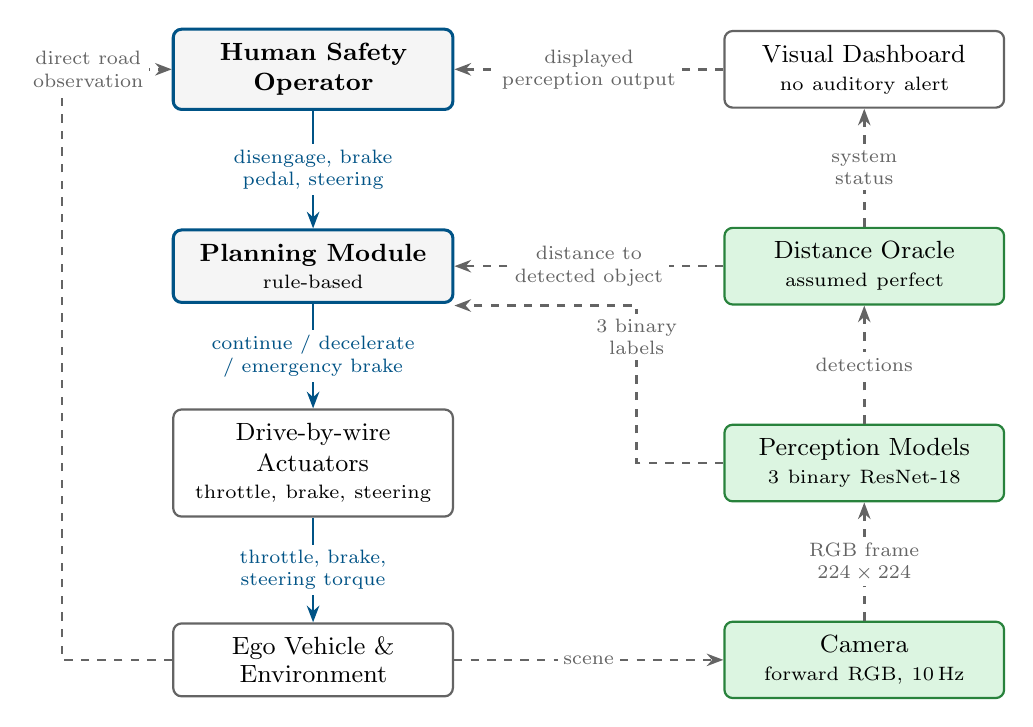
\begin{tikzpicture}[
  ctrl/.style = {rectangle, rounded corners=3pt, draw=mls@blue, fill=mls@lightgray,
                 line width=1.1pt, text width=3.2cm, align=center,
                 font=\small\bfseries, inner sep=5pt},
  proc/.style = {rectangle, rounded corners=3pt, draw=mls@gray, fill=white,
                 line width=0.8pt, text width=3.2cm, align=center,
                 font=\small, inner sep=5pt},
  sens/.style = {rectangle, rounded corners=3pt, draw=mls@green, fill=mls@lightgreen,
                 line width=0.8pt, text width=3.2cm, align=center,
                 font=\small, inner sep=5pt},
  ca/.style   = {-{Stealth[length=6pt]}, mls@blue, line width=1pt},
  fb/.style   = {-{Stealth[length=6pt]}, mls@gray, dashed, line width=0.9pt},
  lbl/.style  = {font=\scriptsize, align=center, inner sep=2pt, fill=white},
]
  \node[ctrl] (op)   at (0,0)      {Human Safety Operator};
  \node[ctrl] (pl)   at (0,-2.5)   {Planning Module\\[-0.1em]{\scriptsize\mdseries rule-based}};
  \node[proc] (ac)   at (0,-5.0)   {Drive-by-wire Actuators\\[-0.1em]{\scriptsize throttle, brake, steering}};
  \node[proc] (ve)   at (0,-7.5)   {Ego Vehicle \&\\[-0.1em]Environment};

  \node[proc] (dash) at (7.0,0)    {Visual Dashboard\\[-0.1em]{\scriptsize no auditory alert}};
  \node[sens] (ora)  at (7.0,-2.5) {Distance Oracle\\[-0.1em]{\scriptsize assumed perfect}};
  \node[sens] (per)  at (7.0,-5.0) {Perception Models\\[-0.1em]{\scriptsize 3 binary ResNet-18}};
  \node[sens] (cam)  at (7.0,-7.5) {Camera\\[-0.1em]{\scriptsize forward RGB, 10\,Hz}};

  \draw[ca] (op.south)  -- (pl.north)   node[lbl,midway] {disengage, brake\\pedal, steering};
  \draw[ca] (pl.south)  -- (ac.north)   node[lbl,midway] {continue / decelerate\\/ emergency brake};
  \draw[ca] (ac.south)  -- (ve.north)   node[lbl,midway] {throttle, brake,\\steering torque};

  \draw[fb] (ve.east)   -- (cam.west)   node[lbl,midway] {scene};
  \draw[fb] (cam.north) -- (per.south)  node[lbl,midway] {RGB frame\\$224\times224$};
  \draw[fb] (per.north) -- (ora.south)  node[lbl,midway] {detections};
  \draw[fb] (ora.north) -- (dash.south) node[lbl,midway] {system\\status};
  \draw[fb] (dash.west) -- (op.east)    node[lbl,midway] {displayed\\perception output};
  \draw[fb] (ora.west)  -- (pl.east)    node[lbl,midway] {distance to\\detected object};
  \draw[fb] (per.west)  -- ++(-1.1,0) |- ([yshift=-0.5cm]pl.east)
                                        node[lbl,pos=0.4] {3 binary\\labels};
  \draw[fb] (ve.west)   -- ++(-1.4,0) |- (op.west)
                                        node[lbl,pos=0.62] {direct road\\observation};
\end{tikzpicture}
\caption{Control structure of the CARLA system. Solid blue arrows are control actions,
dashed grey arrows are feedback. The operator is the higher-level controller and its only
feedback channels are the visual dashboard and direct observation of the road --- there is
no auditory alert and no independent sensor.}
\label{fig:control-structure}
\end{figure}

\subsection{Losses}

{\small
\begin{longtable}{@{}P{1.0cm}P{4.2cm}P{9.8cm}@{}}
\toprule
\textbf{ID} & \textbf{Loss} & \textbf{Why unacceptable} \\
\midrule
\endfirsthead
\toprule
\textbf{ID} & \textbf{Loss} & \textbf{Why unacceptable} \\
\midrule
\endhead
\bottomrule
\endlastfoot
L-1 & Death or serious injury of a pedestrian or other vulnerable road user
    & Irreversible harm to an uninvolved party who has not consented to the risk; the
      dominant societal acceptance criterion for AV testing. \\
L-2 & Death or serious injury of vehicle occupants (ego or third-party)
    & Irreversible harm; also arises from unnecessary hard braking, not only from
      collisions. \\
L-3 & Damage to the ego vehicle, third-party property or infrastructure
    & Reversible but costly; a leading indicator of the mechanisms that cause L-1/L-2. \\
L-4 & Loss of regulatory permission and public trust in the test programme
    & A single publicised incident terminates the programme, so it must be treated as a
      first-class loss rather than a consequence. \\
\end{longtable}}

\subsection{Hazards}

{\small
\begin{longtable}{@{}P{0.9cm}P{11.6cm}P{2.5cm}@{}}
\toprule
\textbf{ID} & \textbf{Hazard} & \textbf{Loss(es)} \\
\midrule
\endfirsthead
\toprule
\textbf{ID} & \textbf{Hazard} & \textbf{Loss(es)} \\
\midrule
\endhead
\bottomrule
\endlastfoot
H-1 & The ego vehicle approaches a pedestrian in its path without decelerating.
    & L-1, L-4 \\
H-2 & The ego vehicle approaches a stationary or slower vehicle ahead within its stopping
      distance without decelerating.
    & L-2, L-3, L-4 \\
H-3 & The ego vehicle enters a signalised intersection while it is required to stop.
    & L-1, L-2, L-3, L-4 \\
H-4 & The ego vehicle applies emergency braking when no obstacle is present.
    & L-2, L-3, L-4 \\
H-5 & The ego vehicle continues in automated mode while its camera input lies outside the
      ODD, so that perception output is untrustworthy and no operator takeover occurs.
    & L-1, L-2, L-3, L-4 \\
\end{longtable}}

\subsection{Unsafe Control Actions}

{\footnotesize
\begin{longtable}{@{}P{1.0cm}P{2.0cm}P{1.9cm}P{1.6cm}P{1.8cm}P{5.5cm}@{}}
\toprule
\textbf{ID} & \textbf{Controller} & \textbf{Control action} & \textbf{UCA type} & \textbf{Hazard(s)} & \textbf{Context in which unsafe} \\
\midrule
\endfirsthead
\toprule
\textbf{ID} & \textbf{Controller} & \textbf{Control action} & \textbf{UCA type} & \textbf{Hazard(s)} & \textbf{Context in which unsafe} \\
\midrule
\endhead
\bottomrule
\endlastfoot
UCA-1 & Planner & Emergency brake & Not provided & H-1
      & A pedestrian is within the critical distance in the ego path. \\
UCA-2 & Planner & Emergency brake & Not provided & H-2
      & A vehicle is ahead within the speed-dependent braking threshold. \\
UCA-3 & Planner & Decelerate / stop at intersection & Not provided & H-3
      & The vehicle approaches a signalised intersection at which stopping is required. \\
UCA-4 & Planner & Emergency brake & Provided when not needed & H-4
      & No road user is within the critical distance and a following vehicle is close
        behind. \\
UCA-5 & Planner & Continue at set speed & Provided & H-5
      & The camera input is outside the ODD (fog, night, unseen town, soiled lens). \\
UCA-6 & Planner & Emergency brake & Provided too late & H-1, H-2
      & The obstacle is only reported after the braking distance at the current speed has
        already been consumed. \\
UCA-7 & Operator & Manual override (brake / steer) & Not provided & H-1, H-2, H-3
      & The automation has failed to act and a collision is imminent. \\
UCA-8 & Operator & Manual override & Provided too late & H-1, H-2
      & Late in a 4-hour monitoring shift, with only a visual dashboard and no auditory
        alert. \\
\end{longtable}}

\subsection{Causal Loss Scenarios}

{\footnotesize
\begin{longtable}{@{}P{1.0cm}P{1.7cm}P{12.3cm}@{}}
\toprule
\textbf{LS-ID} & \textbf{For UCA} & \textbf{Causal scenario (why the UCA occurs)} \\
\midrule
\endfirsthead
\toprule
\textbf{LS-ID} & \textbf{For UCA} & \textbf{Causal scenario (why the UCA occurs)} \\
\midrule
\endhead
\bottomrule
\endlastfoot
LS-1 & UCA-1, UCA-6
     & The pedestrian detector emits a false negative on a nominal in-ODD daytime frame.
       Measured recall is $0.191$, i.e.\ 571 of 706 pedestrian-positive test frames
       produce no detection, so the planner registers ``no pedestrian'' and never
       arms the brake. \\
LS-2 & UCA-2
     & The vehicle detector misses a vehicle ahead (recall $0.800$; 540 of 2\,700 positive
       frames missed), so no deceleration request is generated. \\
LS-3 & UCA-3
     & The traffic-light detector reports only presence, not state. Even a perfect
       detector leaves the planner unable to decide whether stopping is required. \\
LS-4 & UCA-1, UCA-2
     & The camera feed is adversarially perturbed --- either digitally
       ($\ell_\infty$-bounded noise on the frame) or physically (a small patch in the
       scene). A $10\times10$ pixel patch is already sufficient to flip the pedestrian
       output on a compromised model (ASR $=1.00$, V-2). \\
LS-5 & UCA-1, UCA-4
     & Overconfident misclassification: the pedestrian classifier emits a false negative
       while reporting high confidence (mean predicted-class confidence $0.959$ at
       accuracy $0.804$; ECE $=0.156$). The planner records ``no pedestrian, reliable'' and
       no low-confidence fallback is triggered. \\
LS-6 & UCA-5, UCA-1
     & Undetected out-of-ODD input: fog, night or unseen-town frames are processed as if
       in-ODD. Confidence cannot be used as the alarm because the pedestrian model becomes
       \emph{more} confident on OOD inputs ($0.945$ in-ODD $\rightarrow 0.976$ under fog
       and at night). \\
LS-7 & UCA-7, UCA-8
     & Operator vigilance decrement: a 4-hour monitoring shift with a purely visual
       dashboard and no auditory alert delays or suppresses takeover exactly when the
       automation has already failed. \\
LS-8 & UCA-1, UCA-5
     & Training/serving pre-processing skew: an inference pipeline that omits the ImageNet
       normalisation used at training collapses the detectors to a constant negative
       output (observed: vehicle detector 0 positive predictions on 3\,600 frames,
       accuracy $0.250$). Total loss of detection is reported as ordinary,
       high-confidence ``nothing there''. \\
LS-9 & UCA-1
     & Supply-chain data poisoning: 10\,\% of pedestrian-positive training frames carry a
       trigger with a flipped label. Clean-set behaviour remains plausible (recall
       $0.381$) while the trigger achieves ASR $=1.00$, so acceptance testing on clean
       data cannot reveal the backdoor. \\
\end{longtable}}

\subsection{Safety Constraints}

{\footnotesize
\begin{longtable}{@{}P{1.0cm}P{1.5cm}P{8.9cm}P{1.5cm}P{1.4cm}@{}}
\toprule
\textbf{SC-ID} & \textbf{Controls} & \textbf{Safety constraint (requirement)} & \textbf{Level} & \textbf{Verified by} \\
\midrule
\endfirsthead
\toprule
\textbf{SC-ID} & \textbf{Controls} & \textbf{Safety constraint (requirement)} & \textbf{Level} & \textbf{Verified by} \\
\midrule
\endhead
\bottomrule
\endlastfoot
SC-1 & LS-1
     & Pedestrian recall on the in-ODD test set shall be $\geq 0.90$.
     & Model & V-1 \\
SC-2 & LS-2
     & Vehicle recall and traffic-light recall on the in-ODD test set shall each be
       $\geq 0.85$.
     & Model & V-1 \\
SC-3 & LS-4, LS-9
     & Recall drop under FGSM at $\varepsilon=0.05$ shall be $<10$\,pp for every detector,
       and no input-space trigger shall achieve an attack success rate $>1\,\%$.
     & Model & V-2 \\
SC-4 & LS-5
     & ECE on the in-ODD test set shall be $\leq 0.05$ after calibration, and the planner
       shall brake at the cost-optimal threshold $\tau^{*}=1/101$ rather than $0.5$.
     & Model & V-3 \\
SC-5 & LS-6
     & An OOD monitor shall separate in-ODD from out-of-ODD input with
       AUROC $\geq 0.90$, for all three detectors.
     & Model & V-4 \\
SC-6 & LS-6, LS-1
     & On a detected ODD violation, or when the predicted probability lies in the
       ambiguous band around $\theta=0.6$, the system shall limit speed to
       $\leq 15$\,km/h and request operator takeover; if takeover does not occur within
       the takeover budget it shall execute a minimal-risk stop.
     & System & V-5 \\
SC-7 & LS-7
     & The takeover request shall be signalled on an auditory \emph{and} a visual channel;
       continuous monitoring shifts shall be limited and takeover latency shall be
       measured per operator.
     & System & V-5 \\
SC-8 & LS-3
     & The planner shall not derive stop decisions at signalised intersections from the
       presence-only traffic-light detector; a state-aware or map-based input is required.
     & System & V-5 \\
SC-9 & LS-8
     & The deployed inference pre-processing shall be bit-identical to the training
       pre-processing, enforced by an automated equivalence test at every start-up.
     & System & V-5 \\
\end{longtable}}



\clearpage
\section{Safety Case}
\label{sec:safety-case}

\begin{mdframed}[style=claimstyle]
\textbf{Claim:}
\textit{The CARLA autonomous driving system operates safely within its Operational Design Domain as specified.}

\medskip
\textbf{Verdict: the claim is not supported by the evidence in this report.}
\end{mdframed}

\begin{mdframed}[style=subclaim]
\textbf{Argument strategy.}
The claim holds if every hazard in \cref{sec:stpa} is adequately controlled by the safety
constraints derived from it, so the claim is argued by verifying each constraint below:
\textbf{model-level} constraints from the experimental evidence produced across the
exercises, \textbf{system-level} constraints from a design argument. Constraints that
cannot be met are carried to \cref{sec:residual}. Every model-level verdict is valid only
over the ODD region covered by the test suite (\cref{sec:odd}: $0.63$ at $k=3$).
\end{mdframed}

\begin{center}
\small
\begin{tabularx}{\linewidth}{@{}X P{2.1cm} P{2.1cm} P{1.9cm} P{1.9cm}@{}}
\toprule
\textbf{Verification}
& \textbf{Verifies SC(s)}
& \textbf{Loss scenario(s)}
& \textbf{Hazard(s)}
& \textbf{Verdict} \\
\midrule
V-1: In-distribution detection performance
& SC-1, SC-2 & LS-1, LS-2 & H-1, H-2, H-3 & \verdictnotmet \\
V-2: Robustness to perturbations
& SC-3 & LS-4, LS-9 & H-1, H-2 & \verdictnotmet \\
V-3: Calibrated uncertainty
& SC-4 & LS-5 & H-1, H-4 & \verdictnotmet \\
V-4: Out-of-distribution detection
& SC-5 & LS-6 & H-5, H-1 & \verdictpartial \\
V-5: Safe system fallback
& SC-6--SC-9 & LS-3, LS-6, LS-7, LS-8 & H-1--H-5 & \verdictnotmet \\
\bottomrule
\end{tabularx}
\end{center}

% --------------------------------------------------------------- V-1
\subsection{V-1: In-Distribution Accuracy}

\begin{mdframed}[style=subclaim]
\textbf{Verifies:} SC-1, SC-2 \quad \textbf{Hazard(s):} H-1, H-2, H-3 \quad
\textbf{Loss scenario(s):} LS-1, LS-2\\
\textbf{Constraint:} The model achieves sufficient recall when operating within the ODD.\\
\textbf{Metric:} Per-class recall on the in-distribution test set (3\,600 frames,
decision threshold $0.5$).
\end{mdframed}

\begin{mdframed}[style=evidencestyle]
\textbf{Evidence (In-Distribution Detection Performance)}\\

\centering
\small
\begin{tabular}{@{}lcccccc@{}}
\toprule
\textbf{Model} & \textbf{Recall} & \textbf{Precision} & \textbf{F1} &
\textbf{Missed positives} & \textbf{Threshold} & \textbf{Met?} \\
\midrule
Pedestrian    & 0.191 & 0.572 & 0.287 & 571 / 706   & $\geq 0.90$ & \no \\
Traffic light & 0.991 & 0.916 & 0.952 & 24 / 2\,584 & $\geq 0.85$ & \yes \\
Vehicle       & 0.800 & 0.986 & 0.883 & 540 / 2\,700 & $\geq 0.85$ & \no \\
\bottomrule
\end{tabular}\\

\bigskip
\verdictline{\verdictnotmet}
\end{mdframed}

\noindent The pedestrian detector --- the one guarding the most severe loss L-1 --- misses
$81\,\%$ of the frames that contain a pedestrian, yet its accuracy ($0.813$) still looks
acceptable because $80.4\,\%$ of test frames contain no pedestrian. Accuracy is dominated
by the negative class and is therefore not a valid safety metric here, which confirms that
\textbf{recall, not accuracy, is the metric that matters}. The vehicle detector is
similarly mis-tuned in the unsafe direction (precision $0.986$, recall $0.800$: it avoids
nuisance braking at the cost of 540 missed vehicles), while the traffic-light detector
trades false alarms (H-4) for missed stops (H-3) at only $0.916$ precision. Both operating
points must be re-thresholded (see V-3).

\paragraph{Supporting Evidence: Explanation Quality}

Grad-CAM (activations of \texttt{layer4} weighted by their gradients w.r.t.\ the single
output logit) was applied to the Exercise-5 pedestrian detector. It was chosen because it
needs no architectural change, is faithful to the last convolutional stage where spatial
evidence is still present, and yields maps directly comparable across conditions.

\begin{figure}[ht]
\centering
\begin{subfigure}[t]{0.235\linewidth}
  \centering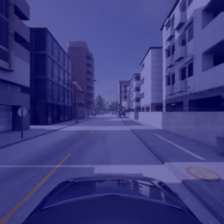
\includegraphics[width=\linewidth]{gradcam_day}
  \caption{In-ODD (daytime)}\label{fig:expl-ped-day}
\end{subfigure}\hfill
\begin{subfigure}[t]{0.235\linewidth}
  \centering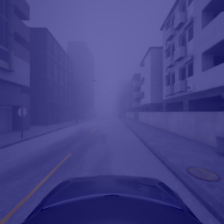
\includegraphics[width=\linewidth]{gradcam_fog}
  \caption{Fog (OOD)}\label{fig:expl-ped-fog}
\end{subfigure}\hfill
\begin{subfigure}[t]{0.235\linewidth}
  \centering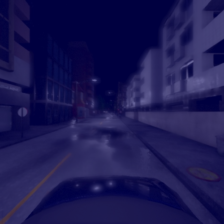
\includegraphics[width=\linewidth]{gradcam_night}
  \caption{Night (OOD)}\label{fig:expl-ped-night}
\end{subfigure}\hfill
\begin{subfigure}[t]{0.235\linewidth}
  \centering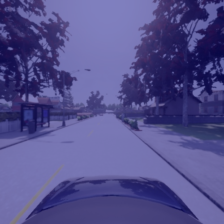
\includegraphics[width=\linewidth]{gradcam_town}
  \caption{Unseen town (OOD)}\label{fig:expl-ped-town}
\end{subfigure}
\caption{Grad-CAM overlays for the pedestrian detector across conditions. Warm colours
indicate high attribution; a uniform blue tint means the map is essentially flat.}
\label{fig:expl-pedestrian}
\end{figure}

\noindent\textbf{Interpretation.} The overlays support LS-1 and LS-6 directly. In-ODD
(\cref{fig:expl-ped-day}) the map is either almost flat or --- as in the correctly
classified frames of \cref{fig:expl-extra} --- concentrated on a building facade in the
upper-left corner, never on a road user: the model reaches correct decisions using
background structure specific to the training town, the textbook symptom of a spurious
correlation and the reason performance transfers so poorly to \texttt{test-town-01}. On
misclassified frames the map collapses into one large blob centred on a \emph{vehicle} in
the middle of the road (\cref{fig:expl-extra}), so the pedestrian decision is being driven
by vehicle-shaped structure. Under fog, night and the unseen town
(\cref{fig:expl-ped-fog,fig:expl-ped-night,fig:expl-ped-town}) attribution becomes
near-uniform --- no evidence is localised anywhere --- yet the model still returns a
confident label. Flat attribution combined with rising confidence (V-4) is precisely the
mechanism of silent failure.


\subsection{V-2: Robustness to Input Perturbations}

\begin{mdframed}[style=subclaim]
\textbf{Verifies:} SC-3 \quad \textbf{Hazard(s):} H-1, H-2 \quad
\textbf{Loss scenario(s):} LS-4, LS-9\\
\textbf{Constraint:} Recall does not degrade substantially under small adversarial
perturbations, limiting the impact of adversarial manipulation of the camera feed.\\
\textbf{Metric:} Recall drop under FGSM at $\varepsilon = 0.05$ (clean $\to$ adversarial).
\end{mdframed}

\begin{mdframed}[style=evidencestyle]
\textbf{Evidence (Adversarial Robustness)}\\

\centering
\small
\begin{tabular}{@{}lcccc@{}}
\toprule
\textbf{Model} & \textbf{Recall (clean)} & \textbf{Recall (FGSM, $\varepsilon=0.05$)} &
\textbf{Drop} & \textbf{Met?} \\
\midrule
Pedestrian    & 0.191 & not measured & --- & \verdictunver \\
Traffic light & 0.991 & not measured & --- & \verdictunver \\
Vehicle       & 0.800 & not measured & --- & \verdictunver \\
\bottomrule
\end{tabular}\\

\bigskip
\textbf{Substitute evidence for the same constraint (input-space perturbation attacks):}\\

\footnotesize
\begin{tabular}{@{}lll@{}}
\toprule
\textbf{Perturbation (pedestrian detector)} & \textbf{Effect} & \textbf{SC-3 limit} \\
\midrule
$10\times10$\,px red trigger, $p=10\,\%$ poison
  & ASR $=1.000$, clean recall $0.381$ & ASR $\leq 0.01$ \\
Fog
  & accuracy $0.797 \rightarrow 0.764$ ($-3.3$\,pp) & --- \\
Night
  & accuracy $0.797 \rightarrow 0.711$ ($-8.6$\,pp) & --- \\
Unseen town
  & accuracy $0.797 \rightarrow 0.752$ ($-4.5$\,pp) & --- \\
\bottomrule
\end{tabular}\\

\bigskip
\verdictline{\verdictnotmet}
\end{mdframed}

\noindent The FGSM measurement specified by the metric was \textbf{not carried out}, so the
$\varepsilon=0.05$ recall drop is unknown and SC-3 is formally unverified for the
digital-attack case. An executable harness (\texttt{adversarial/fgsm\_robustness.py},
$\varepsilon\in\{0.01,0.05,0.1\}$, budget applied in raw pixel space with the ImageNet
normalisation folded into the model) is provided in the repository so the gap can be closed
without re-training; this is the first item of future work.

The second half of SC-3 is, however, decisively \emph{violated}. Poisoning $10\,\%$ of
pedestrian-positive training frames with a $10\times10$ pixel red square and flipping their
label yields an attack success rate of $1.000$: \emph{every} triggered pedestrian-positive
test frame is classified as ``no pedestrian''. The backdoored model retains a clean recall
of $0.381$ --- higher than the honest baseline's $0.191$ --- so no acceptance test on clean
data would raise a flag. That patch is about $0.2\,\%$ of a $224\times224$ frame and could
be realised physically as a sticker on street furniture, which makes LS-4 and LS-9 credible
rather than theoretical. Together with the natural-corruption degradations the available
evidence points unambiguously to non-robustness, so the verdict is recorded as \emph{not
met} rather than merely unverified.


\subsection{V-3: Calibrated Uncertainty}

\begin{mdframed}[style=subclaim]
\textbf{Verifies:} SC-4 \quad \textbf{Hazard(s):} H-1, H-4 \quad
\textbf{Loss scenario(s):} LS-5\\
\textbf{Constraint:} The models provide well-calibrated confidence, so that
low-confidence predictions can trigger fallback behaviour rather than silently
overcommitting.\\
\textbf{Metric:} Expected Calibration Error (ECE, 10 equal-width bins) on the
in-distribution test set; threshold $\leq 0.05$. Temperature $T$ chosen by grid search
over $0.5$--$3.0$ in steps of $0.1$, on validation NLL.
\end{mdframed}

\begin{mdframed}[style=evidencestyle]
\textbf{Evidence (Uncertainty)} --- ECE of the predicted-class confidence,
$T$ from validation NLL:\\

\centering
\footnotesize
\begin{tabular}{@{}lcccccc@{}}
\toprule
\textbf{Model} & \textbf{ECE (single)} & \textbf{$T^{*}$} & \textbf{ECE (scaled)} &
\textbf{Mean conf.} & \textbf{Accuracy} & \textbf{Met?} \\
\midrule
Pedestrian    & 0.156 & 2.9 & 0.056 & 0.959 & 0.804 & \no \\
Traffic light & 0.597 & 3.0 & 0.394 & 0.902 & 0.305 & \no \\
Vehicle       & 0.736 & 3.0 & 0.557 & 0.986 & 0.250 & \no \\
\bottomrule
\end{tabular}

\bigskip
An independent cross-check run on the normalised inference pipeline, scoring the
positive-class probability instead, reaches the same conclusion for all three models
(\cref{tab:ece-cross}).

\bigskip
\verdictline{\verdictnotmet}
\end{mdframed}

\noindent All three models are \textbf{overconfident} in both runs: the signed calibration
gap (mean confidence minus accuracy) is positive for every model, and every ECE value
exceeds the $0.05$ threshold. Temperature scaling helps but does not close the gap; the
best case is the pedestrian detector at $0.056$, still above the limit. The verdict is
therefore invariant to which run is taken as authoritative, which is why both are reported.

\begin{mdframed}[style=cautionstyle]
\textbf{Validity caveat.} The two runs differ and neither is a superset of the other. The
primary run uses the standard predicted-class-confidence definition of ECE, but ran
inference with \texttt{Resize}\,+\,\texttt{ToTensor} \emph{without} the ImageNet
normalisation used at training. That pre-processing skew collapses two of three detectors
to a constant negative output (vehicle: 0 positive predictions on 3\,600 frames, accuracy
$0.250$; traffic light: 81 positive predictions, accuracy $0.305$), so their ECE of $0.74$
and $0.60$ is inflated by the skew, not by miscalibration alone. The cross-check run uses
the correct normalised pipeline but scores the positive-class probability, which penalises
the pedestrian model for being confidently negative. The observation is itself an important
safety result, recorded as LS-8 and RR-5: a silent pre-processing mismatch is sufficient to
disable an entire detector while every prediction still looks confident and well-formed.
\end{mdframed}

\paragraph{Cost-optimal decision threshold.} With $C_{\text{FN}}=100$ and
$C_{\text{FP}}=1$ the two actions have equal expected loss at
$\tau^{*}=C_{\text{FP}}/(C_{\text{FP}}+C_{\text{FN}})=1/101\approx0.0099$, fifty times
lower than the argmax rule. Evaluating
$L=C_{\text{FN}}\cdot\#\text{FN}+C_{\text{FP}}\cdot\#\text{FP}$ on the pedestrian detector:

\begin{center}
\small
\begin{tabular}{@{}lcccc@{}}
\toprule
\textbf{Pedestrian model} & $\boldsymbol{\tau=0.5}$ & $\boldsymbol{\tau=\tau^{*}}$ &
\textbf{FP at $\tau^{*}$} & \textbf{Recall at $\tau^{*}$} \\
\midrule
Uncalibrated ($T=1.0$)       & 70\,600 & 3\,265 & 2\,765 & 0.993 \\
Temperature-scaled ($T=2.9$) & 70\,600 & \textbf{2\,894} & 2\,894 & 1.000 \\
\bottomrule
\end{tabular}
\end{center}

\noindent The lowest loss is calibrated $+$ $\tau^{*}$, a $24\times$ reduction from the
default operating point --- but nearly all of the gain comes from moving the
\emph{threshold}, not from calibrating: $3\,265 \rightarrow 2\,894$ is an $11\,\%$
improvement, whereas $\tau=0.5$ costs $70\,600$ regardless of calibration. At $\tau=0.5$ the
detector predicts ``no pedestrian'' on all 3\,600 frames (recall $0.000$), and calibration
cannot rescue it because temperature scaling is monotone in the logit and so never changes
a decision taken at a fixed threshold. The cost-optimal point does reach perfect recall,
but it flags 2\,894 of 3\,600 frames as pedestrian-positive (accuracy $0.196$), degenerating
into near-permanent braking. \textbf{Neither operating point is deployable}, which is the
quantitative core of the deployment recommendation.

\paragraph{Effect of $T$ on the confidence gate $\theta=0.6$.}
Because $T>0$ preserves the sign of the logit, accuracy is identical at
$T\in\{0.5,1.0,2.0\}$ ($0.7967$ in-ODD). What $T$ changes is how often the constraint ``if
confidence $<\theta$, reduce speed to $\leq15$\,km/h'' fires: $3\,138$ frames at $T=0.5$,
$3\,180$ at $T=1.0$, $3\,228$ at $T=2.0$ (of 3\,600). A small $T$ sharpens the distribution
towards $0$ and $1$ (\cref{fig:hist}) and fires the gate \emph{least often}, so it is the
\textbf{less safe} setting: it suppresses precisely the caution the constraint was written
to produce. Conversely $T=2.0$ fires on $90\,\%$ of frames, making the gate operationally
useless. Accuracy can therefore never verify this constraint on its own; the additional
property that must be measured is calibration of the probability itself, which is what ECE
quantifies.


\subsection{V-4: Out-of-Distribution Detection}

\begin{mdframed}[style=subclaim]
\textbf{Verifies:} SC-5 \quad \textbf{Hazard(s):} H-5, H-1 \quad
\textbf{Loss scenario(s):} LS-6\\
\textbf{Constraint:} An accompanying monitor reliably flags inputs that fall outside the
ODD, preventing silent failure on conditions not covered by training data (fog, night).\\
\textbf{Metric:} AUROC separating the 3\,600 in-ODD test frames from the 10\,800 OOD frames
(fog $+$ night $+$ unseen town); threshold $\geq 0.90$.
\end{mdframed}

\begin{mdframed}[style=evidencestyle]
\textbf{Evidence (Anomaly Detection)}\\

\centering
\small
\renewcommand{\arraystretch}{1.15}
\begin{tabular}{@{}llcl@{}}
\toprule
\textbf{Model used} & \textbf{Detector} & \textbf{AUROC} & \textbf{Met?} \\
\midrule
Vehicle       & MSP (max.\ softmax probability)               & 0.751 & \no \\
Vehicle       & $k$-NN, $k=5$, mean feature distance          & 0.983 & \yes \\
Pedestrian    & not evaluated                                 & ---   & not verified \\
Traffic light & not evaluated                                 & ---   & not verified \\
\bottomrule
\end{tabular}

\bigskip
\textbf{Mean predicted-class confidence per condition} (why MSP fails):\\

\begin{tabular}{@{}lcccc@{}}
\toprule
\textbf{Model} & \textbf{In-ODD} & \textbf{Fog} & \textbf{Night} & \textbf{Unseen town} \\
\midrule
Pedestrian    & 0.945 & 0.976 & 0.976 & 0.958 \\
Traffic light & 0.963 & 0.814 & 1.000 & --- \\
Vehicle       & 0.904 & 0.609 & 0.862 & --- \\
\bottomrule
\end{tabular}\\

\bigskip
\verdictline{\verdictpartial}
\end{mdframed}

\noindent The confidence table explains the result. A classifier's own softmax cannot be
trusted as an OOD signal because nothing in the training objective ties confidence to
familiarity: the pedestrian detector is \emph{more} confident under fog and at night
($0.976$) than in-ODD ($0.945$), so an MSP monitor would flag OOD inputs \emph{less} often
than nominal ones for the most safety-critical detector. Aggregated over all OOD scenarios
the vehicle model's MSP reaches AUROC $0.751$, far below the $0.90$ requirement.

The feature-based $k$-NN detector reaches AUROC $0.983$, comfortably above threshold,
because it measures distance in representation space instead of asking the classifier how
sure it is: a shift that leaves the output layer confident still moves the embedding. Two
caveats keep the verdict at \emph{partial} rather than met. First, it was evaluated for the
vehicle model only, so SC-5's ``for all three detectors'' is not discharged. Second, in this
run the feature extractor was instantiated with random rather than trained weights and the
in-distribution reference set was the test split itself rather than the training split. The
high AUROC is therefore evidence that fog/night/town frames are separable by \emph{some}
feature-space statistic, not yet evidence that the deployed monitor generalises; re-running
with the trained backbone and a training-split reference bank is required before SC-5 can
be claimed.


\subsection{V-5: Safe System Fallback}

\begin{mdframed}[style=subclaim]
\textbf{Verifies:} SC-6, SC-7, SC-8, SC-9 \quad \textbf{Hazard(s):} H-1--H-5 \quad
\textbf{Loss scenario(s):} LS-3, LS-6, LS-7, LS-8\\
\textbf{Constraint:} The system provides a safe fallback when a perception model fails or
operates outside the ODD --- even if a model produces incorrect output, the architecture
limits propagation of the error to harm through fallback behaviour and human oversight.
\end{mdframed}

\begin{mdframed}[style=evidencestyle]
\textbf{Evidence (Design argument)}\\

\textbf{Fallback behaviour defined:} \emph{none is implemented in the system as
specified.} The system description states explicitly that no safety mechanisms beyond the
human operator are deployed. The following four-stage fallback is therefore specified as a
\emph{required design change}, not as existing evidence:

\begin{enumerate}[itemsep=1pt,topsep=2pt,leftmargin=*]
  \item \textbf{Threshold change (SC-4).} Arm braking at $\tau^{*}=1/101$ instead of
        $0.5$, on temperature-scaled probabilities.
  \item \textbf{Confidence gate (SC-6).} Where the probability lies in the ambiguous band
        around $\theta=0.6$, limit speed to $\leq15$\,km/h so that the braking distance
        stays inside the reliable detection range.
  \item \textbf{OOD gate (SC-6).} On a $k$-NN monitor alarm, disable automated speed
        control, issue a takeover request and, if it is not answered within the takeover
        budget, execute a minimal-risk stop at the roadside.
  \item \textbf{Independent stop authority (SC-8).} Derive stop decisions at signalised
        intersections from map data plus a state-aware signal classifier, never from the
        presence-only detector.
  \end{enumerate}

\textbf{Bound on operator takeover.} For the operator to bound H-1 the takeover must
complete within $t_{\text{TOR}} \leq (d_{\text{detect}}-d_{\text{brake}})/v$. At
$v=50$\,km/h $=13.9$\,m/s and $d_{\text{brake}}\approx12$\,m at $0.8\,g$, a usable
detection range of $40$\,m leaves $t_{\text{TOR}}\leq2.0$\,s. Nothing in the design
supports that bound: the alert is visual only, shifts run for four hours, and takeover
latency is never measured (LS-7).

\textbf{System-level constraints addressed by design:} SC-6, SC-7, SC-8, SC-9 are
\emph{specified} above but none is implemented or measured in the current system.\\

\bigskip
\verdictline{\verdictnotmet}
\end{mdframed}

\noindent The decisive argument is structural. A fallback can only bound a hazard if its
failure probability is both small and independent of the failure it is catching. Here
neither holds: the operator shares the same single camera view of the world as the
automation, receives no auditory alert, and --- given a pedestrian recall of $0.191$ --- is
not a fallback for the automation at all but its \emph{primary} detector. Delegating
80\,\% of pedestrian detections to an unmeasured human channel is not a safety argument,
and the constraint cannot be discharged.



\section{Residual Risks and Mitigations}
\label{sec:residual}

\subsection{Residual Risks}

{\footnotesize
\begin{longtable}{@{}P{0.9cm}P{1.1cm}P{8.2cm}P{4.5cm}@{}}
\toprule
\textbf{ID} & \textbf{From} & \textbf{Residual risk (hazard left under-controlled)} & \textbf{Mitigation for the next version} \\
\midrule
\endfirsthead
\toprule
\textbf{ID} & \textbf{From} & \textbf{Residual risk (hazard left under-controlled)} & \textbf{Mitigation for the next version} \\
\midrule
\endhead
\bottomrule
\endlastfoot
RR-1 & V-1
     & H-1 is essentially uncontrolled: the pedestrian detector misses 571 of 706
       positive frames, so the automation contributes almost nothing to pedestrian
       protection. H-2 is partly uncontrolled (540 missed vehicles).
     & Class-balanced or focal loss; oversample pedestrian-positive frames; set the
       operating threshold from a recall target rather than $0.5$; crop-and-zoom
       augmentation for distant pedestrians; move to a detector with localisation. \\
RR-2 & V-2
     & H-1 and H-2 remain open under adversarial input. The FGSM recall drop is unknown,
       and a $10\times10$ pixel trigger achieves ASR $=1.00$ on a poisoned model.
     & Run the provided FGSM harness as an $\varepsilon$-budget acceptance gate;
       PGD adversarial fine-tuning; activation-clustering screening of the training set;
       provenance control and hashing of every training batch. \\
RR-3 & V-3
     & H-1 and H-4 remain open through LS-5: confidence carries no usable information, so
       no confidence-gated fallback can be trusted. The cost-optimal threshold restores
       recall only by braking on $80\,\%$ of frames.
     & Calibrate on a held-out split rather than test; add ensembles or MC dropout for
       epistemic uncertainty; report per-condition ECE; re-tune the cost matrix against
       an achievable false-positive rate. \\
RR-4 & V-4
     & H-5 remains partly open: no OOD monitor is verified for the pedestrian or
       traffic-light detector, and the verified $k$-NN result rests on random features and
       a test-split reference bank.
     & Rebuild the $k$-NN/Mahalanobis bank per model from trained backbone features on
       the \emph{training} split; report per-scenario AUROC and FPR95; add an
       image-quality monitor. \\
RR-5 & V-3 note
     & LS-8 is unmitigated: a silent pre-processing mismatch disables a detector
       completely while every output still looks confident.
     & Serialise the pre-processing with the weights; assert an equivalence test
       against stored reference activations at start-up (SC-9); monitor the
       output-rate distribution for plausibility. \\
RR-6 & ODD
     & $37\,\%$ of 3-way ODD combinations are untested; no frame combines two adverse
       conditions and rain is absent entirely, so no verdict extends there.
     & Collect combinatorial CARLA splits (fog $\times$ night, night $\times$ town,
       rain, dusk) until 3-projection coverage reaches $0.90$. \\
RR-7 & V-5
     & Every hazard H-1--H-5 ultimately relies on an operator whose takeover latency is
       unmeasured, unalerted and subject to a four-hour vigilance decrement.
     & Implement the four-stage fallback of V-5; add auditory takeover alerts; cap shifts
       and add driver-monitoring; measure takeover latency per operator and treat the
       $95$th percentile as the budget in the $t_{\text{TOR}}$ bound. \\
\end{longtable}}

\subsection{Known design limitations}

These follow from the system as specified; no model metric in this report can close them.

{\footnotesize
\begin{longtable}{@{}P{0.9cm}P{11.5cm}P{2.1cm}@{}}
\toprule
\textbf{ID} & \textbf{Limitation} & \textbf{Hazard left open} \\
\midrule
\endfirsthead
\toprule
\textbf{ID} & \textbf{Limitation} & \textbf{Hazard left open} \\
\midrule
\endhead
\bottomrule
\endlastfoot
DL-1 & The traffic-light detector reports presence only, not state, so even at recall
       $0.991$ its high score contributes nothing to intersection safety.
     & H-3 \\
DL-2 & No sensor redundancy: a single camera is the only perception input, so every
       perception fault is a single point of failure with nothing to cross-check it.
     & H-1--H-5 \\
DL-3 & The human operator is the only fallback, is alerted visually only, and works
       4-hour shifts; takeover latency is never measured.
     & H-1--H-5 \\
DL-4 & All training and test data are CARLA renderings, so no claim transfers to real
       camera imagery (sensor noise, motion blur, real material appearance).
     & H-1--H-5 \\
DL-5 & Frames are resized to $224\times224$, destroying the pixel support of distant
       pedestrians --- exactly where early braking matters most.
     & H-1 \\
DL-6 & Binary whole-image classification gives no localisation, so the planner cannot tell
       whether a detected pedestrian is in the ego path or on a sidewalk; the
       assumed-perfect distance oracle hides this gap.
     & H-1, H-4 \\
\end{longtable}}



\section{Deployment Recommendation}
\label{sec:deployment}

\begin{mdframed}[style=subclaim]
\textbf{Recommendation:} \quad
$\square$\ Deploy \quad $\square$\ Deploy with restrictions \quad
$\boxtimes$\ \textbf{Do not deploy}

\medskip
\noindent\textbf{Conditions / restrictions.} No public-road operation, with or without a
safety operator; only closed-course or simulation-in-the-loop testing with no uninvolved
road users present. Re-assessment requires, as a minimum: pedestrian recall $\geq0.90$ and
vehicle recall $\geq0.85$ at a declared threshold (SC-1, SC-2); FGSM recall drop $<10$\,pp
and ASR $\leq1\,\%$ (SC-3); post-calibration ECE $\leq0.05$ on a held-out split (SC-4);
AUROC $\geq0.90$ for \emph{all three} detectors from trained features and a training-split
bank (SC-5); the four-stage fallback implemented with measured takeover latency (SC-6,
SC-7); and 3-projection ODD coverage $\geq0.90$.

\medskip
\noindent\textbf{Justification.} Four of five verifications fail and the fifth is only
partial. V-1 is disqualifying on its own: pedestrian recall is $0.191$ against a $0.90$
requirement, missing $81\,\%$ of the frames containing the road user whose injury is loss
L-1, so H-1 is effectively uncontrolled by the automation. V-2 shows the constraint is not
merely unverified but violated, a $10\times10$ pixel trigger flipping every
pedestrian-positive frame (ASR $=1.00$) while clean-set metrics stay plausible. V-3 shows
all three detectors overconfident beyond the ECE limit before and after temperature
scaling, so no confidence-gated fallback can be trusted, and the cost-optimal threshold
that restores recall to $1.000$ does so by braking on $80\,\%$ of frames. V-4 is only
partial, with MSP at $0.751$ and the pedestrian model growing \emph{more} confident on
out-of-ODD input. V-5 cannot be discharged at all, because the only fallback is a human who
shares the same single camera view, gets no auditory alert, and is in practice the primary
pedestrian detector rather than a backup.

These failures compound rather than offset: an under-performing detector (V-1) whose errors
are indistinguishable from correct outputs (V-3), on inputs whose novelty is not reliably
flagged (V-4), with no independent channel to catch the error (V-5). No restricted envelope
within the declared ODD can be defended on this evidence.
\end{mdframed}



% -------------------------------------------------------- statement of authorship
\clearpage
\thispagestyle{empty}
\begin{center}
  {\large\bfseries\color{mls@blue}Statement of Authorship}
\end{center}

\medskip
I hereby declare that I have independently written the present work and have not used any sources or aids other than
those stated.

Texts, trains of thought, concepts, graphics, etc.\ from external sources that I have directly or
indirectly adopted in my work I have clearly marked as such and provided with complete references
to the respective source. All other content of this work (text parts, figures, tables, etc.)
without corresponding references originates in the copyright sense from me.

I have exclusively used AI systems whose use was approved by the examiner as an aid.

Excluded from the requirement of identification are orthographic or grammatical corrections,
translations, and improvements to formulations that do not alter meaning.

I am aware that AI-generated texts offer no guarantee for the quality of content and text.
I therefore declare that I have used AI systems only as an aid, that I have listed and marked the
AI-generated content, critically reviewed it, and that my independent contribution predominates in
this work.

I confirm that I have fully understood the content of my work and can represent it independently.

\vspace{3cm}

\noindent
\begin{minipage}[t]{0.42\linewidth}
  \rule{\linewidth}{0.4pt}\\[0.2em]{\small Place, Date}
\end{minipage}\hfill
\begin{minipage}[t]{0.42\linewidth}
  \rule{\linewidth}{0.4pt}\\[0.2em]{\small Signature}
\end{minipage}


\clearpage
\appendix

\section{Additional Material}
\label{sec:additional}

\subsection{Reproduction map}

{\footnotesize
\begin{longtable}{@{}P{4.6cm}P{10.4cm}@{}}
\toprule
\textbf{Result in this report} & \textbf{Produced by (run all cells / execute the script)} \\
\midrule
\endfirsthead
\toprule
\textbf{Result in this report} & \textbf{Produced by (run all cells / execute the script)} \\
\midrule
\endhead
\bottomrule
\endlastfoot
Architecture, training curves, class balance (\cref{sec:arch}, \cref{tab:losses})
  & \texttt{Excercise 3/3 Fundamentals.ipynb} \\
Recall / precision / F1, confusion matrices (V-1)
  & \texttt{Excercise 4/4 Model Testing and Validation.ipynb} \\
$k$-projection ODD coverage (\cref{sec:odd})
  & \texttt{odd\_coverage/k\_projection\_coverage.py} \\
Grad-CAM overlays (V-1, \cref{fig:expl-pedestrian}, \cref{fig:expl-extra})
  & \texttt{explainability/explain\_conditions.py},
    \texttt{explain\_correct.py}, \texttt{explain\_errors.py} \\
Backdoor clean recall and ASR (V-2)
  & \texttt{Excercise 5/backdoor\_attack.py} \\
FGSM recall drop (V-2, \emph{pending})
  & \texttt{adversarial/fgsm\_robustness.py} (add \texttt{-{}-limit 100} for the
    100-image subset) \\
Accuracy and confidence-gate counts vs.\ $T$ (V-3, \cref{tab:tempcond})
  & \texttt{Excercise 5/temperature\_scaling.py} \\
ECE, reliability diagrams, $\tau^{*}$ loss table (V-3, primary run)
  & \texttt{Excercise 9/9 Uncertainty Quantification.ipynb} \\
ECE cross-check on the normalised pipeline (V-3, \cref{tab:ece-cross})
  & \texttt{Excercise 8/8 Adversarial ML.ipynb} \\
MSP and $k$-NN AUROC, mean confidences (V-4)
  & \texttt{Excercise 7/7 Anomaly Detection.ipynb} \\
\end{longtable}}

\subsection{Training and validation loss per epoch}

\begin{center}
\small
\begin{tabular}{@{}ccccc@{}}
\toprule
& \multicolumn{2}{c}{\textbf{Pedestrian}} & \multicolumn{2}{c}{\textbf{Traffic light}} \\
\cmidrule(lr){2-3}\cmidrule(lr){4-5}
\textbf{Epoch} & \textbf{Train} & \textbf{Validation} & \textbf{Train} & \textbf{Validation} \\
\midrule
1 & 0.5128 & 0.5690 & 0.1975 & 0.1126 \\
2 & 0.4310 & 0.5949 & 0.0826 & 0.1160 \\
3 & 0.3676 & 0.5181 & 0.0712 & 0.1121 \\
4 & 0.3174 & 0.6950 & 0.0527 & 0.0730 \\
5 & 0.2686 & 0.7138 & 0.0383 & 0.0770 \\
\bottomrule
\end{tabular}
\captionof{table}{Binary cross-entropy per epoch. The pedestrian detector's validation loss
rises from epoch 3 onward while its training loss keeps falling --- overfitting on the
minority class, consistent with the recall failure in V-1. The vehicle detector's curves
were not retained in the notebook output.}
\label{tab:losses}
\end{center}

\subsection{Calibration cross-check on the normalised pipeline}

\begin{center}
\small
\begin{tabular}{@{}lcccc@{}}
\toprule
\textbf{Model} & \textbf{ECE (single)} & \textbf{$T^{*}$} & \textbf{ECE (temp.\ scaled)} & \textbf{Met?} \\
\midrule
Pedestrian    & 0.749 & 3.0 & 0.609 & \no \\
Traffic light & 0.245 & 1.9 & 0.207 & \no \\
Vehicle       & 0.226 & 1.5 & 0.220 & \no \\
\bottomrule
\end{tabular}
\captionof{table}{V-3 cross-check. Inference run with the ImageNet normalisation used at
training, ECE computed on the positive-class probability with $T$ chosen by grid search.
Every value still exceeds the $0.05$ limit, so the V-3 verdict does not depend on which
run is taken as authoritative. The pedestrian figure is high because this definition
penalises a model that is confidently \emph{negative} on $80\,\%$ of frames.}
\label{tab:ece-cross}
\end{center}

\subsection{Per-condition accuracy and confidence-gate counts}

\begin{center}
\small
\begin{tabular}{@{}lccc@{}}
\toprule
\textbf{Split} & \textbf{$T$} & \textbf{Accuracy} & \textbf{Frames with $p<0.6$ (of 3\,600)} \\
\midrule
\texttt{test} (in-ODD)  & 0.5 & 0.7967 & 3\,138 \\
                        & 1.0 & 0.7967 & 3\,180 \\
                        & 2.0 & 0.7967 & 3\,228 \\
\midrule
\texttt{test-fog}       & 0.5 & 0.7636 & 3\,340 \\
                        & 1.0 & 0.7636 & 3\,376 \\
                        & 2.0 & 0.7636 & 3\,454 \\
\midrule
\texttt{test-night}     & 0.5 & 0.7106 & 2\,926 \\
                        & 1.0 & 0.7106 & 3\,017 \\
                        & 2.0 & 0.7106 & 3\,169 \\
\midrule
\texttt{test-town-01}   & 0.5 & 0.7517 & 2\,781 \\
                        & 1.0 & 0.7517 & 2\,840 \\
                        & 2.0 & 0.7517 & 2\,983 \\
\bottomrule
\end{tabular}
\captionof{table}{Exercise-5 pedestrian detector. Accuracy is invariant in $T$ because
dividing a logit by $T>0$ cannot change its sign, so the decision at threshold $0.5$ is
unchanged; only the confidence-gate count moves.}
\label{tab:tempcond}
\end{center}

\subsection{Predicted-probability distributions}

\begin{figure}[ht]
\centering
\begin{subfigure}[t]{0.32\linewidth}
  \centering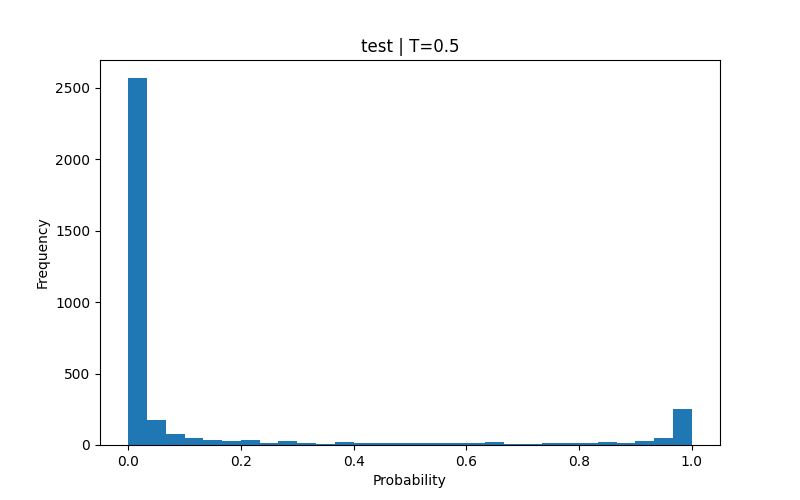
\includegraphics[width=\linewidth]{hist_test_T05}
  \caption{in-ODD, $T=0.5$}
\end{subfigure}\hfill
\begin{subfigure}[t]{0.32\linewidth}
  \centering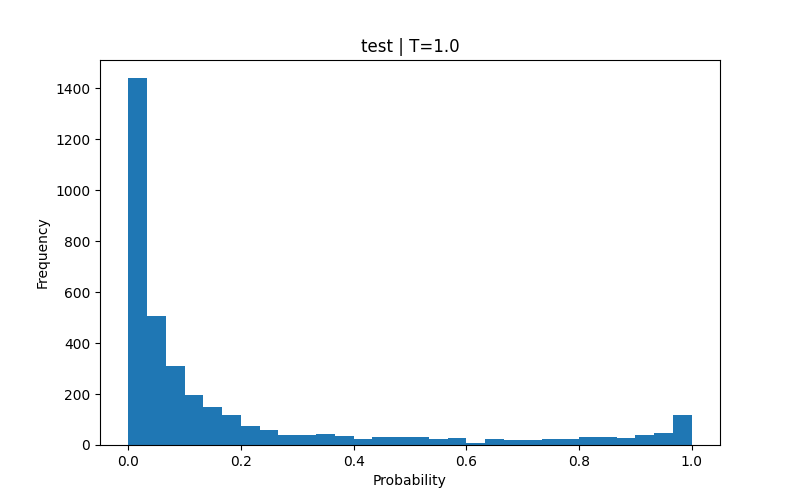
\includegraphics[width=\linewidth]{hist_test_T10}
  \caption{in-ODD, $T=1.0$}
\end{subfigure}\hfill
\begin{subfigure}[t]{0.32\linewidth}
  \centering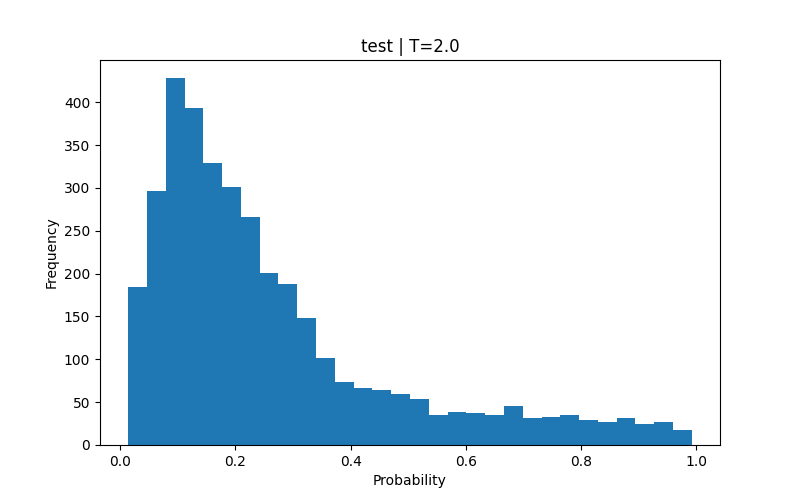
\includegraphics[width=\linewidth]{hist_test_T20}
  \caption{in-ODD, $T=2.0$}
\end{subfigure}

\medskip
\begin{subfigure}[t]{0.32\linewidth}
  \centering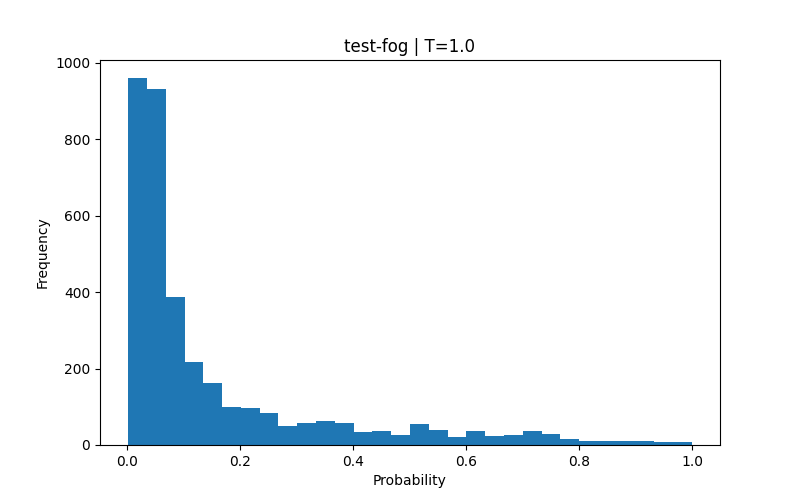
\includegraphics[width=\linewidth]{hist_fog_T10}
  \caption{fog, $T=1.0$}
\end{subfigure}\hfill
\begin{subfigure}[t]{0.32\linewidth}
  \centering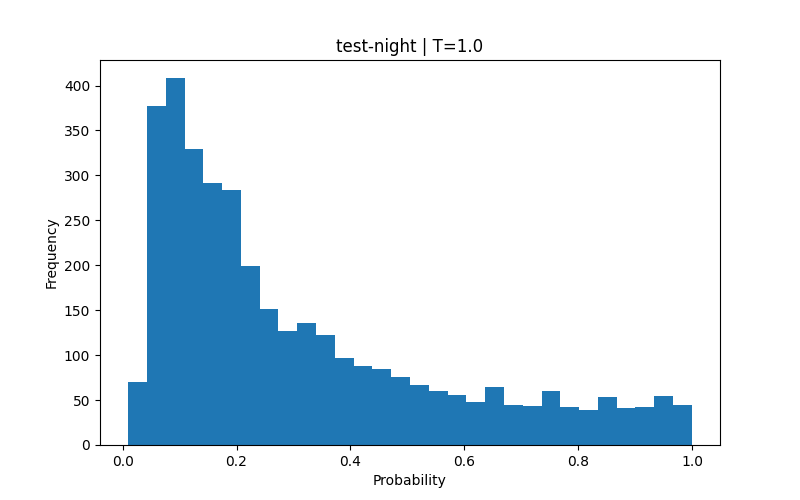
\includegraphics[width=\linewidth]{hist_night_T10}
  \caption{night, $T=1.0$}
\end{subfigure}\hfill
\begin{subfigure}[t]{0.32\linewidth}
  \centering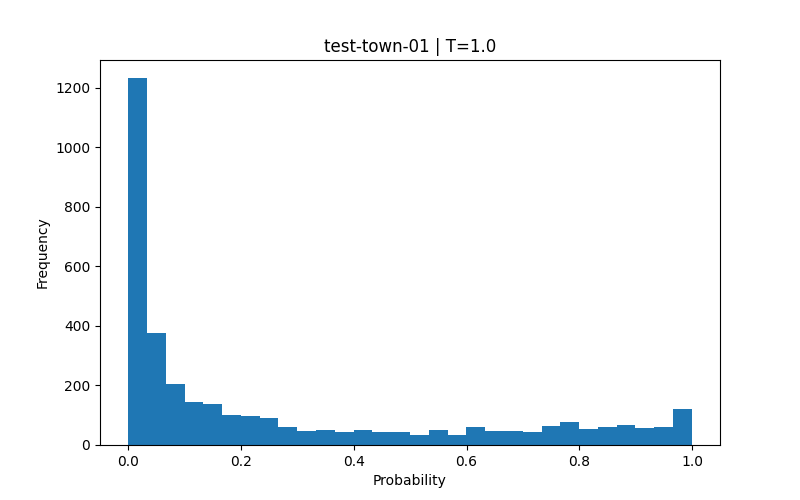
\includegraphics[width=\linewidth]{hist_town_T10}
  \caption{unseen town, $T=1.0$}
\end{subfigure}
\caption{Distribution of the predicted pedestrian probability $p_T$. Raising $T$ pulls mass
away from the extremes towards the centre; lowering it sharpens the distribution towards
$0$ and $1$ and therefore fires the $\theta=0.6$ confidence gate least often. The night and
unseen-town splits carry visibly more mass above $0.6$ than the in-ODD split, i.e.\ the
model is not less confident out of domain.}
\label{fig:hist}
\end{figure}

\subsection{Grad-CAM on correct and misclassified in-ODD frames}

\begin{figure}[ht]
\centering
\begin{subfigure}[t]{0.235\linewidth}
  \centering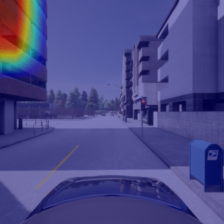
\includegraphics[width=\linewidth]{gradcam_correct_1}
  \caption{correct}
\end{subfigure}\hfill
\begin{subfigure}[t]{0.235\linewidth}
  \centering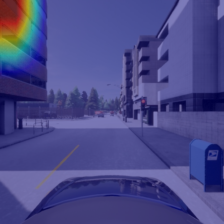
\includegraphics[width=\linewidth]{gradcam_correct_2}
  \caption{correct}
\end{subfigure}\hfill
\begin{subfigure}[t]{0.235\linewidth}
  \centering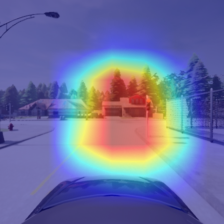
\includegraphics[width=\linewidth]{gradcam_error_1}
  \caption{misclassified}
\end{subfigure}\hfill
\begin{subfigure}[t]{0.235\linewidth}
  \centering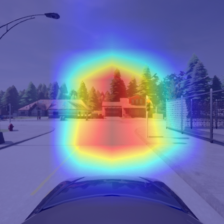
\includegraphics[width=\linewidth]{gradcam_error_2}
  \caption{misclassified}
\end{subfigure}
\caption{Grad-CAM on the in-ODD test split. On correctly classified frames the attribution
sits on a building facade in the upper-left corner, not on any road user --- a spurious
correlation with the training town. On misclassified frames it forms one large blob centred
on a vehicle in the middle of the road, i.e.\ the pedestrian decision is driven by
vehicle-shaped structure. The frames within each pair are temporally adjacent, because the
selection scripts take the first matching frames of the split rather than a random sample;
they are therefore not independent examples.}
\label{fig:expl-extra}
\end{figure}


\end{document}
